\documentclass[a4paper,11pt]{book}
%\documentclass[a4paper,twoside,11pt,titlepage]{book}
\usepackage{listings}
\usepackage[utf8]{inputenc}
\usepackage[spanish]{babel}

% \usepackage[style=list, number=none]{glossary} %
%\usepackage{titlesec}
%\usepackage{pailatino}

%\usepackage[
%backend=biber,
%style=alphabetic,
%sorting=ynt
%]{biblatex}
\usepackage{biblatex}
\addbibresource{bibliografia.bib}
\usepackage{breakcites}

\decimalpoint
\usepackage{dcolumn}
\newcolumntype{.}{D{.}{\esperiod}{-1}}
\makeatletter
\addto\shorthandsspanish{\let\esperiod\es@period@code}
\makeatother


%\usepackage[chapter]{algorithm}
\RequirePackage{verbatim}
%\RequirePackage[Glenn]{fncychap}
\usepackage{fancyhdr}
\usepackage{graphicx}
\graphicspath{./doc/imagenes}
\usepackage{afterpage}

\usepackage{longtable}

\usepackage[pdfborder={000}]{hyperref} %referencia

% ********************************************************************
% Re-usable information
% ********************************************************************
\newcommand{\myTitle}{Aplicación de dietas adaptativas\xspace}
\newcommand{\myDegree}{Grado en ingeniería informática\xspace}
\newcommand{\myName}{Alejandro Olivares del Rey Pierres\xspace}
\newcommand{\myProf}{Juan Julián Merelo Guervós\xspace}
%\newcommand{\mySupervisor}{Put name here\xspace}
\newcommand{\myFaculty}{Escuela Técnica Superior de Ingenierías Informática y de
Telecomunicación\xspace}
\newcommand{\myFacultyShort}{E.T.S. de Ingenierías Informática y de
Telecomunicación\xspace}
\newcommand{\myDepartment}{Departamento de Arquitectura y Tecnología de Computadores\xspace}
\newcommand{\myUni}{\protect{Universidad de Granada}\xspace}
\newcommand{\myLocation}{Granada\xspace}
\newcommand{\myTime}{\today\xspace}
\newcommand{\myVersion}{Version 0.1\xspace}


\hypersetup{
pdfauthor = {\myName (email (en) ugr (punto) es)},
pdftitle = {\myTitle},
pdfsubject = {},
pdfkeywords = {palabra_clave1, palabra_clave2, palabra_clave3, ...},
pdfcreator = {LaTeX con el paquete ....},
pdfproducer = {pdflatex}
}

%\hyphenation{}


%\usepackage{doxygen/doxygen}
%\usepackage{pdfpages}
\usepackage{url}
\usepackage{colortbl,longtable}
\usepackage[stable]{footmisc}
%\usepackage{index}

%\makeindex
%\usepackage[style=long, cols=2,border=plain,toc=true,number=none]{glossary}
% \makeglossary

% Definición de comandos que me son tiles:
%\renewcommand{\indexname}{Índice alfabético}
%\renewcommand{\glossaryname}{Glosario}

\pagestyle{fancy}
\fancyhf{}
\fancyhead[LO]{\leftmark}
\fancyhead[RE]{\rightmark}
\fancyhead[RO,LE]{\textbf{\thepage}}
\renewcommand{\chaptermark}[1]{\markboth{\textbf{#1}}{}}
\renewcommand{\sectionmark}[1]{\markright{\textbf{\thesection. #1}}}

\setlength{\headheight}{1.5\headheight}

\newcommand{\HRule}{\rule{\linewidth}{0.5mm}}
%Definimos los tipos teorema, ejemplo y definición podremos usar estos tipos
%simplemente poniendo \begin{teorema} \end{teorema} ...
\newtheorem{teorema}{Teorema}[chapter]
\newtheorem{ejemplo}{Ejemplo}[chapter]
\newtheorem{definicion}{Definición}[chapter]

\definecolor{gray97}{gray}{.97}
\definecolor{gray75}{gray}{.75}
\definecolor{gray45}{gray}{.45}
\definecolor{gray30}{gray}{.94}

\lstset{ frame=Ltb,
     framerule=0.5pt,
     aboveskip=0.5cm,
     framextopmargin=3pt,
     framexbottommargin=3pt,
     framexleftmargin=0.1cm,
     framesep=0pt,
     rulesep=.4pt,
     backgroundcolor=\color{gray97},
     rulesepcolor=\color{black},
     %
     stringstyle=\ttfamily,
     showstringspaces = false,
     basicstyle=\scriptsize\ttfamily,
     commentstyle=\color{gray45},
     keywordstyle=\bfseries,
     %
     numbers=left,
     numbersep=6pt,
     numberstyle=\tiny,
     numberfirstline = false,
     breaklines=true,
   }
 
% minimizar fragmentado de listados
\lstnewenvironment{listing}[1][]
   {\lstset{#1}\pagebreak[0]}{\pagebreak[0]}

\lstdefinestyle{CodigoC}
   {
	basicstyle=\scriptsize,
	frame=single,
	language=C,
	numbers=left
   }
\lstdefinestyle{CodigoC++}
   {
	basicstyle=\small,
	frame=single,
	backgroundcolor=\color{gray30},
	language=C++,
	numbers=left
   }

 
\lstdefinestyle{Consola}
   {basicstyle=\scriptsize\bf\ttfamily,
    backgroundcolor=\color{gray30},
    frame=single,
    numbers=none
   }


\newcommand{\bigrule}{\titlerule[0.5mm]}


%Para conseguir que en las páginas en blanco no ponga cabecerass
\makeatletter
\def\clearpage{%
  \ifvmode
    \ifnum \@dbltopnum =\m@ne
      \ifdim \pagetotal <\topskip
        \hbox{}
      \fi
    \fi
  \fi
  \newpage
  \thispagestyle{empty}
  \write\m@ne{}
  \vbox{}
  \penalty -\@Mi
}
\makeatother

\usepackage{pdfpages}
\begin{document}
\begin{titlepage}
 
 
\newlength{\centeroffset}
\setlength{\centeroffset}{-0.5\oddsidemargin}
\addtolength{\centeroffset}{0.5\evensidemargin}
\thispagestyle{empty}

\noindent\hspace*{\centeroffset}\begin{minipage}{\textwidth}

\centering

\includegraphics[width=0.9\textwidth]{imagenes/logo.png}\\[1.4cm]

\textsc{ \Large TRABAJO FIN DE GRADO\\[0.2cm]}
\textsc{ INGENIERÍA EN ...}\\[1cm]
% Upper part of the page
% 
% Title
{\Huge\bfseries Titulo del Proyecto\\
}
\noindent\rule[-1ex]{\textwidth}{3pt}\\[3.5ex]
{\large\bfseries Subtitulo del Proyecto}
\end{minipage}

\vspace{2.5cm}
\noindent\hspace*{\centeroffset}\begin{minipage}{\textwidth}
\centering

\textbf{Autor}\\ {Nombre Apellido1 Apellido2 (alumno)}\\[2.5ex]
\textbf{Directores}\\
{Nombre Apellido1 Apellido2 (tutor1)\\
Nombre Apellido1 Apellido2 (tutor2)}\\[2cm]

\includegraphics[width=0.3\textwidth]{imagenes/etsiit_logo.png}\\[0.1cm]
\textsc{Escuela Técnica Superior de Ingenierías Informática y de Telecomunicación}\\
\textsc{---}\\
Granada, mes de 2023
\end{minipage}
%\addtolength{\textwidth}{\centeroffset}
%\vspace{\stretch{2}}
\end{titlepage}



\chapter*{}
%\thispagestyle{empty}
%\cleardoublepage

%\thispagestyle{empty}

\cleardoublepage
\thispagestyle{empty}

\begin{center}
{\large\bfseries Aplicación de dietas adaptativas: Adaptando tu alimentación a tus necesidades}\\
\end{center}
\begin{center}
Alejandro Olivares del Rey Pierres\\
\end{center}

%\vspace{0.7cm}
\noindent{\textbf{Palabras clave}: frontend, framework, git, backend, dataset, project management, crawler, design thinking}\\

\vspace{0.7cm}
\noindent{\textbf{Resumen}}\\

A todo el mundo nos ha ocurrido el problema de tener muchos ingredientes en la despensa, al final acabas olvidando algunos, como tomate escondido en el frigorífico o el típico tarro que tenemos al fondo de la despensa detrás de ingredientes que se terminan usando mucho más. Cuando se va a utilizar un ingrediente que sabemos que tenemos, y lo encontramos caducado e inutilizable sentimos una frustración por no recordar su existencia, además de tener que volver a comprarlo en el supermercado. Por ello, en este proyecto se analizará una posible solución a esta problemática por la que todos hemos pasado. Para un correcto desarrollo del proyecto, se utilizará una metodología ágil permitiendo obtener las ventajas del uso de este tipo de metodología. Se necesitarán perfilar los usuarios a los que va dirigida la solución del problema, haciendo uso del diseño orientado al usuario, pensando específicamente que quiere dicho usuario. Para guardar el progreso y llevar una correcta gestión se utilizarán herramientas de control de versiones. Además de analizar los diversos lenguajes que se pueden utilizar para el desarrollo del software, seleccionando el más adecuado dependiendo del tipo de implementación que se realice en el proyecto. 

Los contenidos incluidos en la memoria son:
\begin{enumerate}
    \item Introducción: Una breve introducción al los problemas alimentarios que existen en nuestro país y la descripción del problema a resolver.
    \item Estado del arte: Un vistazo a aplicaciones similares que puedan ser competencia directa con la solución que se va a desarrollar.
    \item Metodología: Descripción de la metodología a seguir en el proyecto, con las principales claves de la metodología ágil que se buscan seguir en el proyecto, las historias de usuario que han servido de guía a lo largo del mismo, user journeys, perfiles de usuarios objetivo de la aplicación y una descripción detallada de los objetivos a seguir. Además se incluye una descripción de design thinking que recoge el proceso seguido para el desarrollo del proyecto.
    \item Planificación. Se recoge la planificación del proyecto desde el inicio del proyecto hasta la elección de la metodología, se expone la dificultad de la planificación siguiendo una mentalidad ágil centrada en las necesidades del usuario, poniendo como punto de partida el desarrollo de la infraestructura del proyecto y como siguiente objetivo la funcionalidad para resolver el problema del usuario.
    \item Implementación: Sección dedicada a la justificación de cada decisión técnica tomada, desde el lenguaje del proyecto hasta el tipo de solución planteada, añadiendo también las decisiones relativas a la infraestructura del proyecto.
    \item Recetas. Explicación de la obtención de recetas, su la manera de guardarlas y acceder a ellas y explicación de la solución diseñada para encontrar recetas en la base de datos, añadiendo consideraciones iniciales de la funcionalidad que resuelve el problema a tratar, algoritmo utilizado y breve explicación de la implementación.
    \item Prototipo. Explicación del uso de prototipo, junto con el diseño de cada parte que lo compone desde la  interfaz, con un diseño inicial y la explicación de la implementación de la misma añadiendo pequeñas funcionalidades para aumentar la usabilidad de la misma, hasta el desarrollo del backend haciendo uso de un framework, estableciendo las conexiones entre el frontend y el backend.
    \item Pruebas. Descripción de los test realizados a las vistas de la aplicación que ven los usuarios para encontrar recetas y viajes por la aplicación de los usuarios descritos.
    \item Análisis del despliegue. Análisis de como desplegar la aplicación para que sea accesible para todos los usuarios desde el sofá de su casa y explicación del diseño de la infraestructura que se utilizará en el despliegue.
    \item Costes: Desglose de gastos en la producción de la aplicación
    \item Conclusiones: Consideraciones finales del proyecto y trabajos futuros.
\end{enumerate}
\cleardoublepage


\thispagestyle{empty}


\begin{center}
{\large\bfseries Adaptative diet app: Adapting your diet to your needs}\\
\end{center}
\begin{center}
Alejandro, Olivares del Rey Pierres \\
\end{center}

%\vspace{0.7cm}
\noindent{\textbf{Keywords}: frontend, framework, git, backend, dataset, project management, crawler, design thinking}\\

\vspace{0.7cm}
\noindent{\textbf{Abstract}}\\

Everyone has had the problem of having a lot of ingredients in the pantry, in the end you end up forgetting some, like tomatoes hidden in the fridge or the typical jar we have at the back of the pantry behind ingredients that end up being used much more. When we are going to use an ingredient that we know we have, and we find it expired and unusable we feel frustrated for not remembering its existence, in addition to having to buy it again at the supermarket. Therefore, this project will analyze a possible solution to this problem that we have all gone through. For a correct development of the project, an agile methodology will be used, allowing to obtain the advantages of the use of this type of methodology. It will be necessary to profile the users to whom the solution to the problem is directed, making use of the user-oriented design, thinking specifically about what the user wants. Version control tools will be used to keep the progress and to manage it correctly. In addition to analyzing the various languages that can be used for software development, selecting the most appropriate depending on the type of implementation to be carried out in the project.

The contents included in the memory are:
\begin{enumerate}
    \item Introduction: A brief introduction to the food problems that exist in our country and the description of the problem to be solved.
    \item State of the art: A look at similar applications that could be in direct competition with the solution to be developed.
    \Methodology: Description of the methodology to be followed in the project, with the main keys of the agile methodology to be followed in the project, the user stories that have served as a guide throughout the project, user journeys, profiles of target users of the application and a detailed description of the objectives to be followed. It also includes a description of design thinking that reflects the process followed for the development of the project.
    \item Planning. The planning of the project from the beginning of the project until the choice of the methodology, the difficulty of the planning is exposed following an agile mentality focused on the user's needs, putting as a starting point the development of the project infrastructure and as the next objective the functionality to solve the user's problem.
    \item Implementation: Section dedicated to the justification of each technical decision taken, from the language of the project to the type of solution proposed, adding also the decisions related to the project infrastructure.
    \item Recipes. Explanation of how to obtain recipes, how to save and access them and explanation of the solution designed to find recipes in the database, adding initial considerations of the functionality that solves the problem to be addressed, algorithm used and brief explanation of the implementation.
    \item Prototype. Explanation of the use of prototype, along with the design of each part that composes it from the interface, with an initial design and explanation of the implementation of the same adding small features to increase the usability of it, to the development of the backend using a framework, establishing the connections between the frontend and backend.
    \item Tests. Description of the tests performed to the views of the application that users see to find recipes and journeys through the application of the described users.
    \item Deployment analysis. Analysis of how to deploy the application so that it is accessible to all users from the sofa at home and explanation of the design of the infrastructure to be used in the deployment.
    \item Costs: Breakdown of expenses in the production of the application.
    \item Conclusions: Final considerations of the project and future work.
\end{enumerate}

\chapter*{}
\thispagestyle{empty}

\noindent\rule[-1ex]{\textwidth}{2pt}\\[4.5ex]

Yo, \textbf{Alejandro Olivares del Rey Pierres}, alumno de la titulación Grado en ingeniería informática de la \textbf{Escuela Técnica Superior
de Ingenierías Informática y de Telecomunicación de la Universidad de Granada}, con DNI 77166527D, autorizo la
ubicación de la siguiente copia de mi Trabajo Fin de Grado en la biblioteca del centro para que pueda ser
consultada por las personas que lo deseen.

\vspace{6cm}

\noindent Fdo: Alejandro Olivares del Rey Pierres

\vspace{2cm}

\begin{flushright}
Granada a 11 de Noviembre de 2023.
\end{flushright}


\chapter*{}
\thispagestyle{empty}

\noindent\rule[-1ex]{\textwidth}{2pt}\\[4.5ex]

D. \textbf{Juan Julián Merelo Guervós}, Profesor del Área de ATC del Departamento ICAR de la Universidad de Granada.

\vspace{0.5cm}

\textbf{Informan:}

\vspace{0.5cm}

Que el presente trabajo, titulado \textit{\textbf{Aplicación de dietas adaptativas,  Adaptando tu alimentación a tus necesidades}},
ha sido realizado bajo su supervisión por \textbf{Juan Julián Merelo Guervós}, y autorizamos la defensa de dicho trabajo ante el tribunal
que corresponda.

\vspace{0.5cm}

Y para que conste, expiden y firman el presente informe en Granada a 11 de Noviembre de 2023.

\vspace{1cm}

\textbf{Los directores:}

\vspace{5cm}

\noindent \textbf{Juan Julián Merelo Guervós}

\chapter*{Agradecimientos}
\thispagestyle{empty}

       \vspace{1cm}


A toda la gente que me ha apoyado en el desarrollo de este trabajo.


%\frontmatter
%\tableofcontents
%\listoffigures
%\listoftables
%
%\mainmatter
%\setlength{\parskip}{5pt}

\chapter{Introducción}

\section{Motivación}
En la actualidad, debido a una gran concienciación impartida por diferentes organismos orientados a la salud, ha aumentado la preocupación por mantener una alimentación saludable y equilibrada. Sin embargo, la gran mayoría de personas no tienen los conocimientos suficientes como para elaborar una dieta adaptada a sus necesidades individuales. Ya no solo estamos hablando de personas que buscan bajar peso, sino de personas que tienen algún tipo de intolerancia o alergia alimentaria.

Según la Fundación de Seguridad Alimentaria (FSA), en el mundo existen unas 520 millones de personas con este tipo de problemas alimentarios. Solo en España se estima que entre el 1-3\% de los adultos y un 4-6\% de los niños padecen algún inconveniente al consumir determinados alimentos. Además, debemos diferenciar a las personas con intolerancias alimentarias de las que sufren alergias. Ya que no tienen los mismos efectos aunque a primera vista sean parecidos. Las alergias se producen cuando el sistema inmune entra en contacto con el alérgeno, mientras que las intolerancias están ligadas a la dificultad para digerir determinados alimentos.\cite{FSA}

Cualquier persona sabe qué es una dieta, ya que todos nos alimentamos cada día. La palabra ``dieta'' se refiere al conjunto de alimentos que ingerimos. Sin embargo, no todo el mundo lleva una dieta equilibrada. Existen múltiples tipos de dietas, como omnívora, vegetariana, vegana, paleo, mediterránea, entre otras, las cuales se diferencian por los alimentos que se consumen.
Es un error común pensar que simplemente al comer de manera saludable se está siguiendo una dieta equilibrada. Para lograr una dieta equilibrada, es necesario consumir todos los nutrientes esenciales que el cuerpo necesita para mantener una salud óptima. Una dieta equilibrada se caracteriza por ser variada, moderada y proporcionada.

Cuando hablamos de variedad, nos referimos a la inclusión de alimentos de todos los grupos: frutas, verduras, cereales, legumbres, carnes, pescados, etc. Por supuesto, hay dietas que excluyen ciertos alimentos; en esos casos, se debe buscar una fuente alternativa de nutrientes. Por otro lado, una dieta debe ser moderada, lo que significa que se deben ingerir las cantidades necesarias de nutrientes sin excederse.

\section{Descripción del problema}
A todo el mundo nos ocurre el tener un montón de ingredientes en la despensa sin saber que hacer con ellos, que se terminan acumulando o caducando, haciendo que sea un derroche de dinero. El problema que se quiere resolver con el desarrollo de esta aplicación es el mal aprovechamiento de los ingredientes que se tienen por casa y el desconocimiento de determinadas recetas que solventen esa mala gestión.

El proyecto va dirigido a usuarios que cuentan con recursos económicos limitados, como un estudiante con un presupuesto ajustado, o personas con movilidad reducida que no puedan permitirse acudir al supermercado cada vez que les falte un ingrediente. 

Pero el uso de esta aplicación no está limitado a estos usuarios descritos, sino que puede ser utilizada por cualquier persona que quiera aprovechar los ingredientes que tengan sueltos por la cocina.

En primer lugar, necesitamos conocer a fondo el problema descrito, para comprender toda la complejidad que pueda tener. Pensando un poco es posible encontrar mucha profundidad a la hora de resolver el problema, por ejemplo, que se entiende por ingrediente o que ingredientes tiene todo el mundo en su casa. Estas preguntar irán surgiendo a medida que avance el desarrollo del proyecto.

Para resolver el problema descrito se utilizarán las mejores prácticas dentro de un enfoque ágil.

\section{Objetivos}
\begin{enumerate} 
    \item Búsqueda básica de recetas. El usuario debe ser capaz de encontrar recetas utilizando los ingredientes que desee.
\end{enumerate}
\chapter{Estado del arte}
Después de una investigación inicial en este campo buscando en diversos blogs de nutrición como \emph{HealthLine}\cite{Healthline2022} y revistas como \emph{Bussines Insider}\cite{BusinessInsider2021} y \emph{The Guardian}, donde se habla de aplicaciones que permiten desde desarrollar una dieta utilizando recetas publicadas por la comunidad o simplemente con los ingredientes que tenemos en nuestro frigorífico. 

Una de las más interesantes de las que se trata es \href{https://www.yummly.com}{\emph{Yummly}}, una aplicación disponible tanto en \emph{iOS} como en \emph{Android} que se adapta a las necesidades individuales de cada persona, incluyendo intolerancias alimentarias \cite{TheGuardian2016}. Esta ofrece un plan gratuito que permite buscar recetas, recomendaciones personalizadas, una lista de la compra. Además cuenta con un plan de pago que cuesta 4,99\$/mes, que incluye la creación de dietas personalizadas, información nutricional de las recetas, un motor de búsqueda por ingredientes que permite filtrar por ingredientes, alergias o tipo de dieta. Pero, desafortunadamente, no está disponible en España. 

Una aplicación quizá más conocida es \href{https://cookpad.com/es/home}{\emph{Cookpad}}, esta es una de las aplicaciones más descargadas de \emph{Apple Store} y \emph{Google Play} en la sección de cocina. Una de sus características principales es su comunidad, donde es posible compartir recetas y fotos de tus creaciones. Es posible usar esta aplicación de manera gratuita pero cuenta con algunas limitaciones. Por otra parte, la versión pro cuesta 2,99\$/mes y entre las funcionalidades que ofrece se encuentran planes de menús semanales elaborados por nutricionistas.

Otra de las aplicaciones más interesantes que se encontraron fue \href{https://www.eatthismuch.com/}{EatThisMuch}.Esta es una aplicación web, también disponible para \emp{Android} e \emph{iOS}, que permite generar una dieta de manera automática basándose en:
\begin{itemize}
    \item Las calorías que se quieren ingerir al día.
    \item El número de comidas que se desea realizar.
    \item El tipo de dieta que se quiere generar.
\end{itemize}
\emph{Eat This Much} tiene una versión gratuita abierta al usuario. Al generar la dieta es posible cambiar el plato aleatoriamente entre los que se recomiendan. Pero, el principal problema se basa en que la personalización de la dieta es muy general, sin tener en cuenta las intolerancias del usuario. De la misma manera, ofrecen una suscripción orientada a profesionales y entrenadores permitiendo que estos recomienden generen las dietas a sus clientes de manera totalmente personalizada. Esta suscripción cuesta 79,00\$/mes y solo incluye servicio para diez clientes, cada cliente extra costará 4\$/mes. 

La última aplicación de la que se hablará es \href{https://happyforks.com/}{\emph{HappyForks}}, que se trata de una herramienta que permite monitorizar una gran cantidad de valores nutricionales. Contando con una gran cantidad de utilidades para controlar una dieta ajustándose a las necesidades del usuario y una gran base de datos llena de recetas. Una de las utilidades que ofrecen permite analizar recetas y productos mostrando los ingredientes para no causar alergias al usuario. 

El GED indica la cantidad de calorías que un individuo debe consumir para abastecer los requerimientos energéticos. Si el gasto corresponde a la ingesta de alimentos, mantendrá su peso. De lo contrario, si la ingesta supera al requerimiento, ganará peso. El gasto energético no solo corresponde a actividades fisiológicas, sino que también depende de las actividades físicas que desarrolle el individuo. Se deben tener en cuenta los siguientes mecanismos: 
\begin{itemize}
    \item Metabolismo basal
    \item Actividad dinámica específica de los alimentos
    \item Termogénesis inducida por el ejercicio
\end{itemize}

El metabolismo basal se trata de la cantidad de energía necesaria para realizar los procesos vitales estando en reposo. Una manera de calcularlo es multiplicando 24kcal por el peso del individuo en kilogramos. El resultado sería la cantidad de energía que necesitaría una persona para sobrevivir 24 horas estando completamente en reposo. 

La actividad dinámica específica de los alimentos, se refiere a la cantidad de calorías que quema una persona al masticar digerir y absorber los alimentos. El valor oscila entre un 6\% y un 10\% dependiendo de cuanto se haya ingerido y del gasto energético basal.

Por último, hay que tener en cuenta el consumo de calorías cuando se hace ejercicio, ya que en los esfuerzos físicos se consume gran cantidad de energía. Dependiendo del nivel de actividad del individuo, se consumirán más calorías. 
\begin{table}[h]
    \begin{center}
        \begin{tabular}{| c | r |}
            Actividad & Gasto energético \\ \hline
            Sedentario & 1,2 \\
            Leve & 1,375 \\
            Moderada & 1,55 \\
            Intensa & 1,725 \\
            Extrema & 1,9 \\ \hline
        \end{tabular}
        \caption{Tabla 1: factor de actividad física}
        \label{tab:FAF}
    \end{center}
\end{table}

La fórmula de Harris-Benedict aprovecha los parámetros introducidos anteriormente, además de otros valores individuales como la edad (años), peso (kg), talla (cm), etc... Para calcular el gasto energético en reposo. Se debe tener en cuenta el sexo del individuo \cite{GER}
\begin{equation}
    Varones:GER = 66,5+(13,75*peso)+(5,08*talla)-(6,78*edad)
\end{equation}
\begin{equation}
    Mujeres:GER = 65,51+(9,56*peso)+(1,85*talla)-(4,68*edad)
\end{equation}

Otra fórmula que permite calcular el GER es la ecuación de Mifflin-St Jeor, desarrollada en 1990, es considerada más precisa que la ecuación Harris-Benedict. También considera el peso (kg), altura (cm), edad (años) y el sexo del individuo \cite{CARRASCO2007}
\begin{equation}
    Varones:GER = (10 * peso) + (6.25 * altura) - (5 * edad) + 5
\end{equation}
\begin{equation}
    Mujeres:GER = (10 * peso) + (6.25 * altura) - (5 * edad) - 161
\end{equation}

Por otra parte, la fórmula de Katch-McArdle solo consta de una ecuacuón tanto para hombres, mujeres, edad y estatura. Esto simplifica el cálculo del metábolismo básal usando solo la cantidad de masa magra. En primer lugar se debe conocer el valor de grasa que tiene el individuo. Si, por ejemplo, tiene un 22\% de grasa entonces consta de un 78\% de masa magra (kg) que se sustituirá en la ecuación \cite{Katch-McArdle}
\begin{equation}
    TMB = 370 + (21,6 * masa)
\end{equation}.

Hay que tener en cuenta que cada fórmula está calculando el gasto energético en reposo, a esto hay que multiplicarle el factor de actividad que se expone en la \autoref{tab:FAF}.
\chapter{Descripción de la metodología}
En este capítulo se describirá la metodología utilizada en el desarrollo a lo largo del proyecto.

\section{Marco ágil}
Debido a las limitaciones de la gestión de proyectos, a finales de los 90 se empezó a utilizar una metodología ágil. Pero no fue hasta 2001 que un grupo de expertos desarrolla el ``Manifiesto por el Desarrollo Ágil de Software''. Donde se especificaron los doce principios clave para el desarrollo de software. A partir de ese punto, cada vez han ido surgiendo más modelos ágiles.

Este proyecto se centrará en el uso de la metodología \emph{Scrum}'. Que es uno de los modelos más utilizados actualmente en el desarrollo de software. Este divide el trabajo en ``Sprints'', intervalos de tiempo en el que un equipo trabaja en un conjunto de tareas definidas con anterioridad. Este marco ofrece una gran flexibilidad para adaptarse a cambios en función de las necesidades del proyecto. Además, al dividir el proyecto en iteraciones más pequeñas se hace más manejable, permitiendo que el desarrollo sea más eficiente.

\section{User Journeys}

En primer lugar se enfocará el software a un estudiante que cuenta con un presupuesto ajustado al mes y no puede permitirse el lujo de comprar en el supermercado todos los días. Dicho estudiante se siente frustrado por no ser capaz de controlar sus gastos en el supermercado y que ciertos ingredientes que no utiliza asiduamente le caduquen en la despensa. Por casualidad descubre el software desarrollado en este proyecto y se lo descarga. Una vez descargado abre la aplicación e introduce los ingredientes que tiene en su despensa. El estudiante podrá encontrar a su disposición diferentes recetas que realizar con los ingredientes introducidos. Una vez seleccionada la receta, el usuario puede comprobar los detalles de la misma.

Otro tipo de usuario al que se orienta este software es una persona mayor que no se encuentra en disposición de ir al supermercado cada vez que le faltan ingredientes y tiene una despensa limitada. De pronto escucha la existencia de la aplicación y se dispone a probarla. Después de descargarla, con dificultad debido a sus achaques de la edad y a su dificultad para entender las nuevas tecnologías, la abre. En primer lugar debe introducir los ingredientes que tiene por casa y aunque encuentra cierta dificultad sustituir una nota de papel, con esfuerzo consigue hacer un inventario de sus ingredientes. La aplicación en este momento le podrá empezar a sugerir recetas con los ingredientes que tiene en su despensa. Después de elegir una receta, puede comprobar los detalles de la misma con detenimiento.

\section{Planificación}
En todo proyecto es muy importante saber que se está haciendo en todo momento y lo que se hará a continuación. Es uno de los puntos, y ventajas, más importantes de la metodología ágil. Por ello, en esta sección se especificará la planificación del proyecto\:
\begin{enumerate}
    \item Establecer el alcance.
    \item Inicio del desarrollo.
    \item Encontrar recetas.
    \item Sustituir ingredientes.
\end{enumerate}

\subsection{Establecer el alcance}
En todo proyecto, ya sea desarrollo software o construir un edificio necesita una planificación. Por ello es muy importante especificar el problema a resolver. En este caso, facilitar a los usuarios el proceso de encontrar recetas que se adapten a los ingredientes que tienen en su despensa. En primer lugar, se han especificado los objetivos a seguir durante el desarrollo del proyecto. Sentar las bases del proyecto ayuda a tener una orientación sobre que hacer en cada momento. 

\subsection{Inicio del desarrollo}
Antes de lanzarse a programar hay que hacer una serie de análisis previos y resolver ciertas cuestiones algunas de ellas son:
\begin{enumerate}
    \item ¿Para que plataforma está orientado el software?
    \item ¿En que lenguaje se realizará?
    \item ¿Se usará una herramienta de control de versiones?
\end{enumerate}
Este paso en la planificación es extremadamente importante, ya que determinará el marco de desarrollo bajo un lenguaje específico que no se puede escoger a la primera de cambio ya que cada uno cuenta con una serie de ventajas y desventajas a tener en cuenta en el proyecto. Aunque estas cuestiones serán resueltas en un capítulo posterior. 

\subsection{Encontrar recetas}
Este es el primer objetivo del software a desarrollar, que permitirá ayudar a los usuarios definidos anteriormente a encontrar recetas que contengan los ingredientes con los que cuentan el usuario. Además, en este punto es necesario definir que tipo de ingredientes son los que tiene cualquier persona en su casa, como por ejemplo: Agua, sal o aceite. Y conforme avance el desarrollo de este objetivo habrá que resolver ciertas cuestiones, como la anterior, que vayan surgiendo. 

\subsection{Sustituir ingredientes}
También se planifica una de las posibles mejoras a seguir una vez se haya completado el desarrollo del proyecto. En este caso se permitiría que se recomendasen recetas a las que les falta uno o varios ingredientes pero es posible sustituirlos de manera coherente con otros ingredientes con los que sí cuenta el usuario. Pero esto es solo una posible mejora para el futuro del software, teniendo que analizar la viabilidad una vez completado el objetivo anterior. 

\section{Github}
\emph{Github} es una herramienta de control de versiones que permite hacer uso de \emph{issues} y \emph{milestones}. Permitiendo llevar tanto los registros de los diferentes cambios que se hacen en el proyecto como un seguimiento con una correcta metodología. Al inicio del proyecto se crean una serie de \emph{issues} que actuan como historias de usuario, donde se identifica el problema a resolver desde el punto de vista de un usuario. En este caso se detalla el problema de querer encontrar recetas con una serie de ingredientes limitados. Los objetivos del proyecto se detallan como \emph{milestones}, siendo estos un \emph{PMV} (producto mínimo viable) que podrá ser entregado al usuario final. A medida que avanza el desarrollo del proyecto se irán creando diversos \emph{issues} que perfilarán el software final. El uso de esta herramienta es muy eficaz en equipos de desarrollo, ya que permite ver en que está trabajando cada integrante viendo que \emph{issues} tiene asignados. Además de permitir que existan varios equipos, cada uno trabajando en una \emph{feature} del software mediante el uso de \emph{branches}. Una vez que está lista, se hace un \emph{Pull Request} donde un desarrollador revisa el código en busca de posibles errores y una vez que todo está en orden se puede mezclar con la rama principal del proyecto. Además, a lo largo del proyecto se establecerán una serie de test que faciliten la integración continua en el software. Detectando cualquier fallo que pueda haber, de antemano, en el código o incompatibilidad con alguna actualización de dependencias. En \emph{Github} se conoce como ``Github Actions'' y, aunque, es posible hacerlos uno mismo existen infinidad de acciones creadas por otros usuarios.

Para concluir esta sección se quiere aclarar que aunque se haya explicado el uso de \emph{Github} en la metodología, en el capítulo siguiente se explicará la elección de esta herramienta sobre otras que hacen una función similar como \emph{Gitlab} o \emph{BitBucket}.
\chapter{Planificación}
En este tercer capítulo se narrará la planificación seguida en el proyecto, desde la definición del problema a resolver hasta la especificación de las metodologías que se utilizarán en el proyecto. 

\section{Introducción}
En el apartado de introducción se detalla la motivación del proyecto, exponiendo los motivos que llevan al desarrollo del proyecto, además se determina que se considera como ``dieta equilibrada'', ya que no todo el mundo tiene el mismo concepto y, adicionalmente, que se considera una ``dieta variada''. 

Por otra parte, se describe el problema desde el punto de vista de los clientes de la aplicación. El problema que se va a resolver es la necesidad que tiene el usuario para encontrar nuevas recetas, o recordar antiguas, utilizando los ingredientes a su disposición. 

Una vez descrito el problema, fue necesario describir a quien se dirige la solución, se determinó que existen dos tipos de cliente a los que se resuelve la necesidad:
\begin{enumerate}
    \item Estudiante
    \item Persona mayor
\end{enumerate}

\section{Estado del arte}
En este capítulo se definen las principales soluciones existentes similares a lo que se busca desarrollar. Se realizó una búsqueda de aplicaciones que pudieran ser parecidas o con una funcionalidad que sea una solución al problema planteado. 

Se encontraron algunas aplicaciones, en blogs de nutrición y revistas \cite{Healthline2022}\cite{TheGuardian2016}\cite{BusinessInsider2021}, que cumplen los requisitos especificados antes, la mayoría son de pago o imponen restricciones a la hora de escoger ingredientes que se utilicen en la búsqueda de recetas. 

Se han detallado las más relevantes o parecidas que se han encontrado.

\section{Metodologías}
En esta sección inicialmente se describe el concepto de marco ágil y las ventajas que se aprovecharán en el desarrollo del proyecto. 

Para el proyecto se plantea el uso de \emph{design thinking}, realizando una pequeña investigación leyendo diversos artículos académicos\cite{wolniak2017design}\cite{thoring2011understanding} que han servido de guía para obtener un entendimiento del concepto de \emph{design thinking} y sus etapas en el desarrollo. Además, se ha especificado el avance en las primeras etapas del proyecto.

La etapa de empatizar con el usuario objetivo se completa pensando en las necesidades que hay que cubrir del usuario. Especificando el viaje del usuario (\emph{user journey}) en la aplicación. Un \emph{user journey} es una herramienta que permite representar paso a paso el proceso que necesita el usuario para alcanzar su objetivo, en este caso encontrar una receta que se adapte a él. \cite{gasparini2015perspective}

Para definir a los usuarios se utiliza la metodología de persona, que permite definir al usuario por medio de una serie de información planteada por medio de preguntas para conocer a fondo al cliente, tanto sus necesidades como sus motivaciones. 

Las preguntas propuestas para el perfilado del usuario permiten entender las necesidades de los clientes potenciales y abasteciéndolos de las funcionalidades o servicios que necesitan.

El proyecto más complejo que el desarrollar una aplicación, es muy importante llevar una correcta gestión del mismo. Para llevar a cabo esa gestión se utiliza \emph{git}, una herramienta de control de versiones que permite trabajar siguiendo una mentalidad ágil resolviendo poco a poco \emph{issues}.

Existen diferentes herramientas que permiten el uso de \emph{git}, se utiliza \emph{Github} por ser la herramienta con la que he trabajado y tengo mayor experiencia en su uso. Pero existen otras herramientas como \emph{Jira} o \emph{Gitlab} en las que tengo menos experiencia.

En la gestión del proyecto se han afrontado algunos desafíos como la correcta creación de \emph{issues} que definan de manera corta un problema o desafío que se necesita resolver para continuar el desarrollo. La definición de \emph{milestones} y que se espera de cada hito también ha supuesto un desafío en esta etapa del proyecto, debido a la poca experiencia que poseía al abordar el proyecto con una mentalidad ágil.

En un punto del desarrollo del \emph{milestone} se desarrolló una parte del proyecto de manera prematura, utilizando una rama para ello. Para afrontar el problema de manera organizada, se abrieron \emph{pull request} lo más atómicos posibles con el objetivo de cerrar los \emph{issues} relativos a este milestone, dejando pendientes los prematuros. Una vez completados todos los \emph{issues} se tomó la decisión de dejar la rama abierta sin mezclar y extraer los cambios realizados para cerrar los problemas abordados. Para ello, se utiliza la operación \emph{cherry-pick}, siendo mejor opción que eliminar la rama y tener que repetir los cambios para solventar los \emph{issues}. Desde una nueva rama con los cambios extraídos de la problemática, se mezclaron con la rama principal sin inconvenientes.

En la planificación del proyecto se tomó la decisión de especificar únicamente los primeros \emph{milestones} del proyecto debido a la imposibilidad de conocer el camino que tomará el desarrollo siguiendo una mentalidad ágil.
\chapter{Implementación}
En todo proyecto existen una serie de decisiones que marcan el avance del proyecto. En este capítulo se describirán, detalladamente, las justificaciones de cada decisión que se tome durante el desarrollo del mismo. Otorgando tanto al lector como a cualquier desarrollador que busque continuar este proyecto, un entendimiento de porqué se han tomado dichas decisiones.

\section{Herramientas de control de versiones}
Como se explicó en capítulos anteriores, \Gls{git} es una herramienta de control de versiones muy poderosa que permite mantener una organización en los cambios realizados en el código de un proyecto por medio de \emph{issues} y \emph{commits}.

Es posible trabajar con \Gls{git} localmente, pero se consiguen mejores resultados al utilizar una plataforma en línea para almacenar estos cambios. Para mantener la coherencia en los cambios del proyecto es necesario elegir una plataforma para el control de versiones. Las dos plataformas consideradas son \href{https://github.com/}{Github} y \href{https://about.gitlab.com/}{GitLab}. 

Dichas plataformas son muy parecidas, dificultando la elección de una de ellas objetivamente. Ambas permiten la gestión del proyecto por medio de un repositorio remoto y están basadas en \Gls{git}. La mayor diferencia que existe entre ambas es el objetivo para el que se utilizan. GitHub es una plataforma colaborativa que ayuda a revisar y gestionar el código remotamente. Mientras que GitLab está más enfocado a proyectos de DevOps y CI/CD. \cite{VCS2022}

En el proyecto se utiliza GitHub por ser la única herramienta de control de versiones  

\section{Herramientas de integración continua}
La integración continua (CI) es un proceso de desarrollo de software que permite al equipo de desarrollo realizar \emph{builds} consistentes, añadiendo test que permitan comprobar que las funcionalidades desarrolladas funcionen como se espera. Los tres pasos esenciales de la integración continua son: Construir, testear y mezclar.

Después de una investigación, de diferentes artículos\emph{online}, en el cambo de los \emph{framework} de integración continua más populares actualmente se deben valorar diferentes soluciones posibles para la implementación de la integración continua. \cite{CIKumar2023}\cite{CITaylor2023}\cite{CIRoddewig2023}

Se consideran las siguientes herramientas como herramientas de CI:
\begin{enumerate}
    \item GitHub Actions
    \item CircleCI
\end{enumerate}

Las mencionadas anteriormente cumplen los dos requisitos, CircleCI cuenta con un plan regido por créditos de ejecución en el primer caso, mientras que GitHub Actions es completamente gratuito. Se utilizará CircleCI por salir de la zona de confort y aprender una nueva herramienta de CI, y adicionalmente, GitHub Actions de ser necesario su uso como soporte, en caso de agotar los créditos mensuales de CircleCI. 

\section{Lenguaje del proyecto}
Para el desarrollo de la solución, de cualquier tipo, es necesario definir un lenguaje de programación. 

\Gls{python} es un lenguaje interpretado, es decir, es un interprete quien traduce línea a línea en tiempo de ejecución el programa a lenguaje máquina. Es un lenguaje flexible, con una sintaxis legible, siendo muy parecida al inglés. Además, cuenta con gran cantidad de módulos indexados y de fácil acceso que le dan esa flexibilidad mencionada anteriormente.

Se elige este lenguaje por ser con el que más experiencia cuento para realizar cualquier tipo de implementación que necesite el proyecto de manera eficaz.

\section{Gestor de dependencias}
En el proyecto es necesario utilizar un gestor de dependencias que resuelva la problemática de la gestión de módulos y bibliotecas externas del proyecto, para facilitar la colaboración en el proyecto y brindar una reproducibilidad en diferentes sistemas y momentos. 

Como opciones se considera Poetry, ya que el lenguaje en el que se implementará el proyecto es \Gls{Python}, y son sencillos de utilizar. Las mejores prácticas en la gestión de dependencias de \Gls{Python} es el uso de pip. Esta herramienta instala las dependencias de manera global, por ello se habla también de aislar los entornos de \Gls{python} para separar las dependencias de un proyecto de otro, teniendo que añadir herramientas extra. 

Se escoge Poetry por ser un gestor de dependencias sencillo que permite gestionar las dependencias de manera sencilla dentro de un entorno virtual por proyecto, para asegurar la reproducibilidad.

\section{Gestor de tareas}
Se considera Poetry e Invoke como gestor de tareas por su simplicidad y completitud. Poetry es mucho más simple y está enfocado a la gestión de dependencias, aunque pueden ejecutar tareas con la librería ``subprocess'' de \Gls{python}. Sigue siendo un gestor de dependencias. 

En conclusión, se elige Invoke como gestor de dependencias por su simplicidad y potencial. Se ajusta mejor a las necesidades del proyecto para lanzar test, siendo también muy intuitivo implementar las tareas, ya que se incluyen en un fichero ``tasks.py'' escrito en \Gls{python}.
\chapter{Recetas}
En este capítulo se detallará todo lo relativo al \href{https://github.com/Slowmybrosh/TFG-DietPlanner/milestone/3}{\emph{\gls{milestone}}} ``Encontrar recetas'', que tiene como objetivo solucionar al usuario la necesidad de encontrar recetas utilizando exclusivamente los ingredientes seleccionados por el usuario.

\section{Fuente de recetas}
Para la obtención de recetas, se obtendrán de la famosa página de recetas \href{https://cookpad.com/es/home}{Cookpad}. Donde la comunidad puede subir cualquier receta. Habiendo mucha variedad de recetas, permitiendo obtener una base de datos variada. Estas recetas se deberán cargar en una base de datos.

El robot de \href{https://www.blueprism.com/es/}{BluePrism}, utiliza un reconocimiento del código fuente, similar a un \emph{\gls{crawler}}, de la página permitiendo seleccionar los elementos deseados de cada una. Inspeccionando la página se pueden analizar una serie de atributos para identificar inequívocamente algunos elementos.

Los pasos que se han seguido para obtener recetas son:
\begin{enumerate}
    \item Buscar diferentes recetas de diferentes tipos (pescado, carne, verduras, etc...)
    \item Obtener los enlaces de dichas recetas
    \item Filtrar los enlaces para evitar los repetidos
    \item Acceder a cada receta y recuperar
    \begin{enumerate}
        \item Nombre
        \item Ingredientes
        \item Pasos
    \end{enumerate}
    \item Formar un fichero en formato \gls{JSON} (JavaScript Object Notation)
\end{enumerate}

Para la función de buscar recetas de diferentes tipos, se lanza un navegador web con la dirección de inicio de \href{https://cookpad.com/es/home}{Cookpad}, al buscar cualquier cosa utilizando el cuadro de búsqueda. La dirección a la que se consulta la petición es la siguiente: \emph{buscar/verduras?event=search.history&order=recent}, con un simple vistazo se puede identificar que la petición en este caso fue ``verduras''. Sabiendo esto, para buscar por tipo de receta se han compuesto las direcciones url de manera dinámica, evitando pasos extra a la hora de realizar esta búsqueda inicial. 

\begin{figure}[H]
    \centering
    \fbox{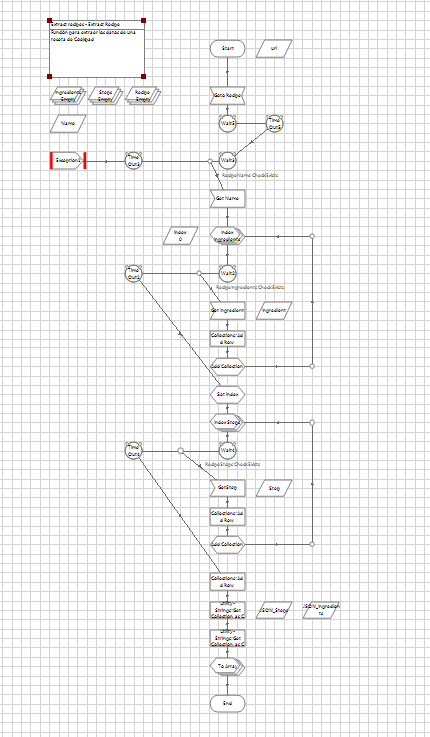
\includegraphics[width=100mm,scale=1]{./doc/imagenes/Extract_recipe.png}}
    \caption{Función para extraer enlaces}
    \label{fig:links}
\end{figure}

En el paso de obtención de la receta, se identifica el nombre de la receta. Utilizando la herramienta de modelado de aplicación que trae incorporada BluePrism. Con ella se puede seleccionar el elemento de la página que se desea extraer y automáticamente se extrae información relevante para la identificación como el identificador del elemento, las clases CSS del mismo, su ruta XPATH, etc... El nombre de las recetas como elemento no es único, al ser una lista de recetas habrá muchas coincidencias que se quieran extraer. Para ello se utiliza el atributo \emph{match\_index}, si se selecciona el primer resultado de la página se obtendría el primer nombre. BluePrism permite recuperar atributos dinámicos, en la función el número de coincidencia itera entre uno y diez para obtener diez recetas de cada tipo. Con la coincidencia del elemento, se extrae el enlace y se guarda en una colección que se pasará a la función para extraer recetas. 

\begin{figure}[H]
    \centering
    \fbox{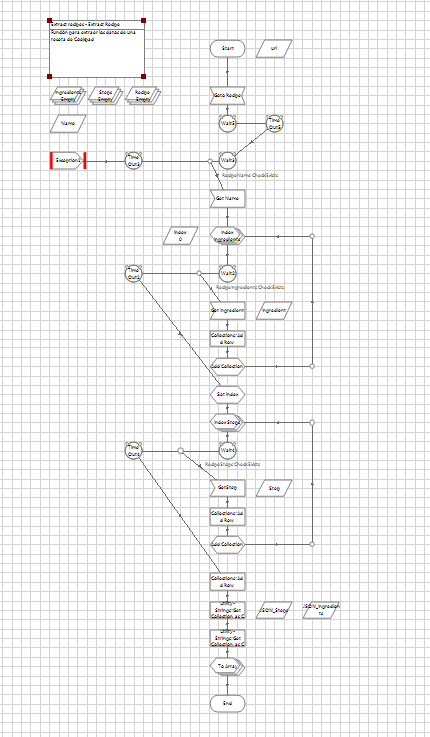
\includegraphics[width=75mm,scale=1]{./doc/imagenes/Extract_recipe.png}}
    \caption{Función para extraer recetas}
    \label{fig:recipe}
\end{figure}

Una vez obtenidos todos los enlaces, puede que haya repetidos por coincidir en la categoría de carne y verduras a la vez, es necesario hacer un filtrado muy sencillo que elimine los enlaces repetidos. 

La función que extrae la receta de la página, obtiene el nombre teniendo en cuenta que es el primer \emph{h1} de la página. Los ingredientes y los pasos se tratan de listas ordenadas, fáciles de extraer. Cada ingrediente tienen un identificador \emph{ingredient} seguido de una cadena de números. BluePrism puede utilizar \emph{wildcards} para identificar elementos de la página web, de la misma manera que al extraer una lista de enlaces, se itera por los ingredientes hasta que no haya más. Con los pasos se sigue el mismo razonamiento, valiéndose de un selector \gls{CSS} para extraer los pasos iterando sobre ellos hasta que no hay más. 

\begin{figure}[H]
    \centering
    \fbox{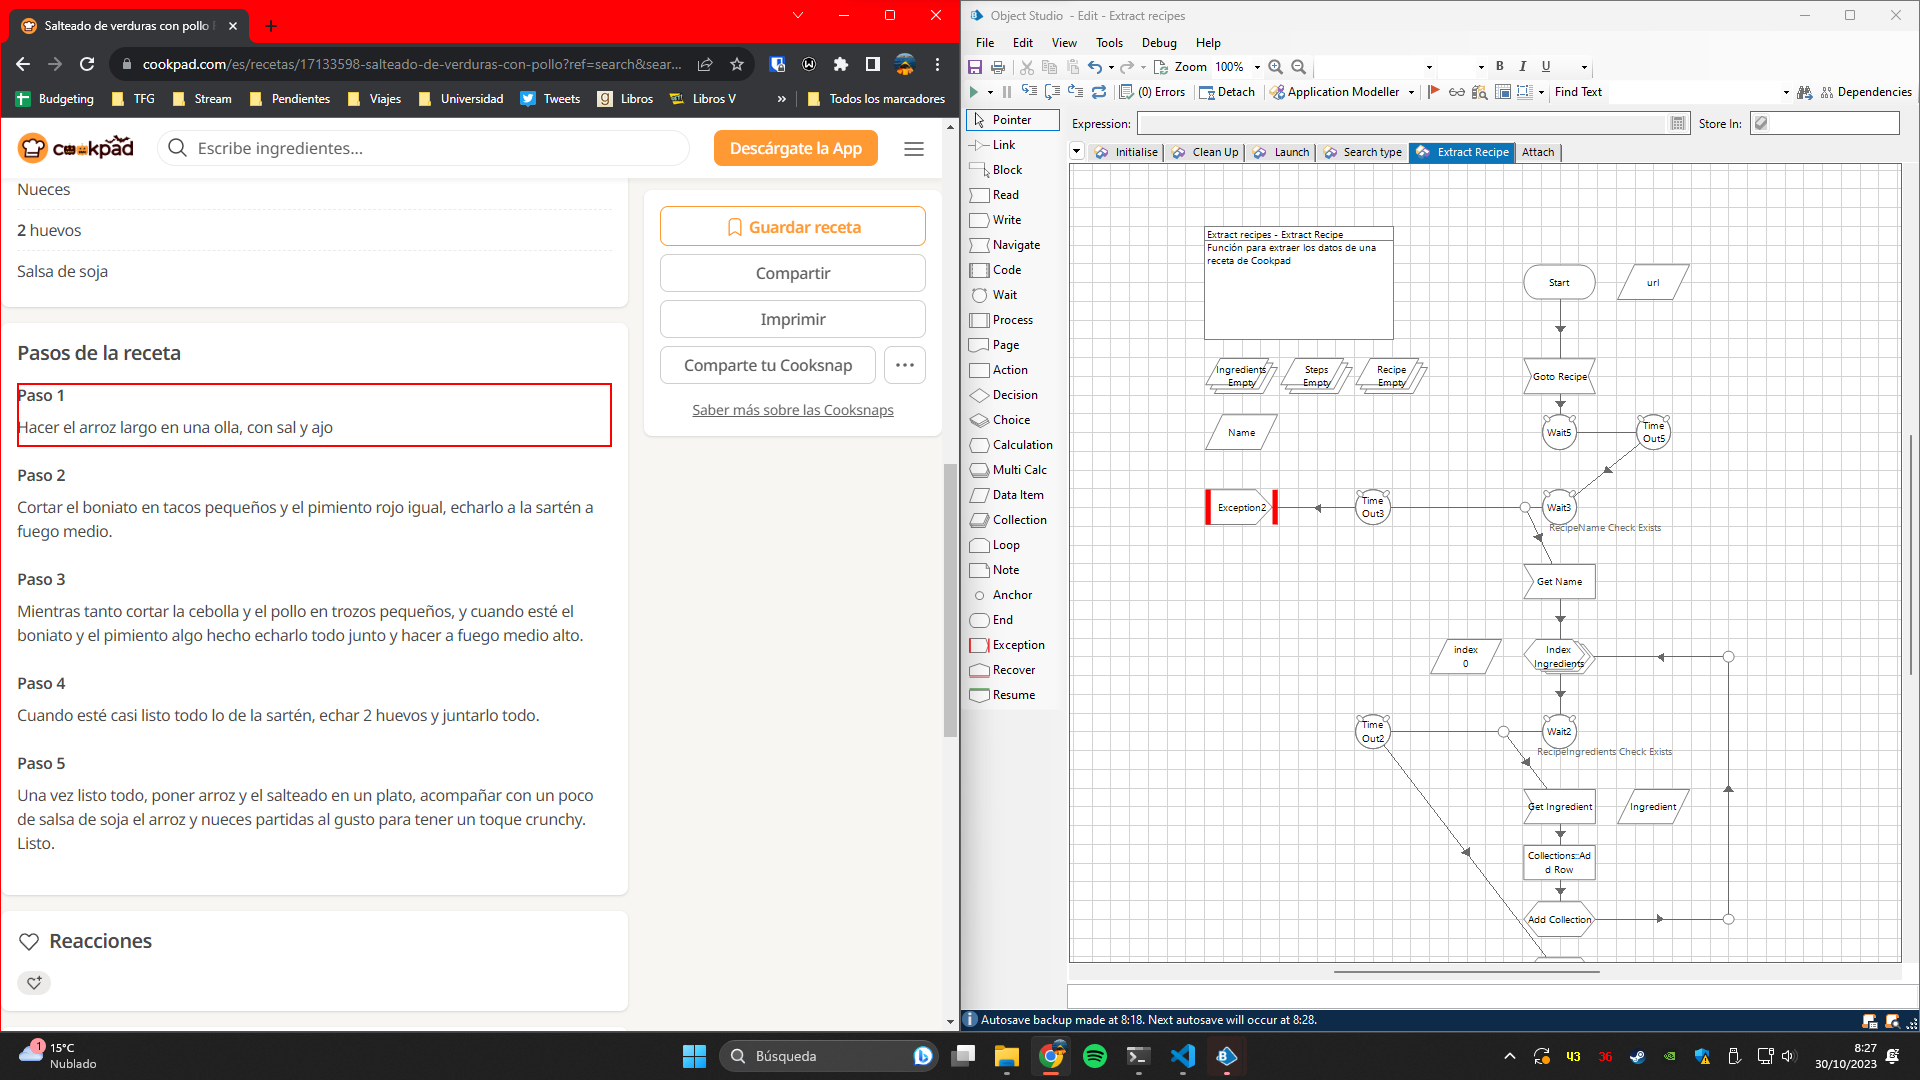
\includegraphics[width=100mm,scale=1]{./doc/imagenes/identify_step.png}}
    \caption{Identificar los pasos de la receta}
    \label{fig:steps}
\end{figure}


Para que constituya una fuente de información uniforme, la colección de recetas se guarda como un fichero \gls{JSON} que puede ser fácilmente recuperado y transformado en cualquier otro formato.

El proceso de ejecución del robot lleva tiempo, ya que el identificar los ingredientes a través de una expresión regular toma entre diez y veinte segundos. Los demás pasos son relativamente menos costosos en cuestión de tiempo. El robot tardó aproximadamente cuatro horas en obtener sesenta y dos recetas con todos los elementos mencionados. La ventaja de haber utilizado este proceso de obtención de recetas es que se puede ampliar en el futuro a conveniencia, aunque hay que tener en cuenta el tiempo que tarda el robot en obtener recetas.

\newpage
\section{Gestión de las recetas en la aplicación}

Para insertar los datos en la aplicación, se insertan en una base de datos relacional para aprovechar la relación que existe entre una receta y los ingredientes que contiene. Permitiendo identificar rápidamente que ingredientes lleva una receta, pudiendo gestionar de manera sencilla los requisitos para realizar una receta. 

Se utiliza un pequeño \gls{script} para insertar los datos desde sus respectivos ficheros a la base de datos siguiendo el siguiente esquema
\begin{figure}[h!]
    \centering
    \fbox{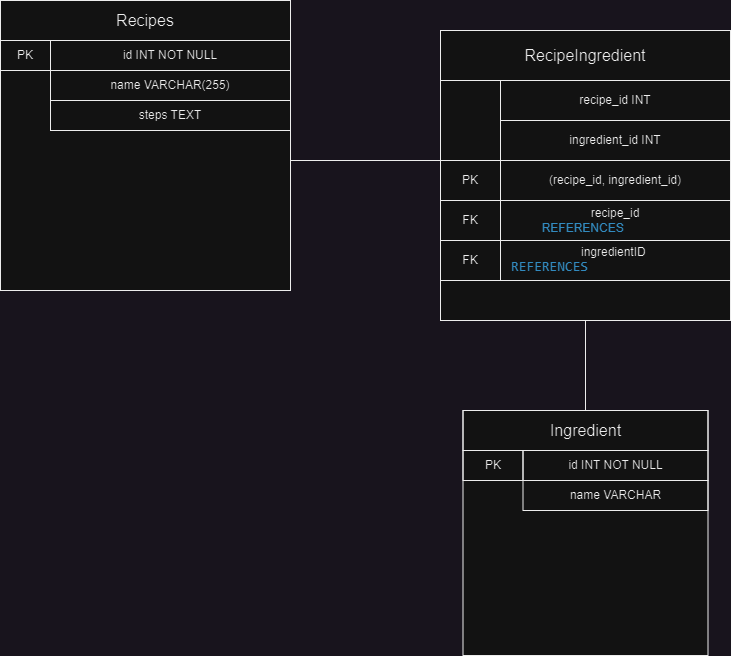
\includegraphics[width=100mm,scale=1]{./doc/imagenes/db.drawio.png}}
    \caption{Esquema de la \gls{base}}
    \label{fig:scheme}
\end{figure}

\newpage
\section{Encontrar recetas}
El primer problema que se pretende resolver con la publicación del proyecto es permitir a los usuarios encontrar recetas, ya sea por aprovechar los ingredientes de su despensa o porque no recuerdan con exactitud los ingredientes de una receta o sus pasos.

\subsection{Consideraciones iniciales}
Antes de explicar como se ha resuelto el problema debemos hacer unas consideraciones iniciales que se han tomado en cuenta en la etapa de modelización del problema.

Por ejemplo, existen ciertos tipos de ingredientes que todo el mundo tiene en casa, por ello no se consideran como restricciones a la hora de encontrar una receta. Estos son
\begin{enumerate}
    \item Agua
    \item Sal
    \item Pimienta
    \item Aceite
    \item Vinagre
\end{enumerate}

Otra consideración importante es que no se tiene en cuenta la cantidad de cada ingrediente que tiene el usuario en casa. Por ejemplo, puede introducir en el buscador que cuenta con macarrones y tomate frito, obtendrá la receta de ``Macarrones con tomate''. Pero a la hora de cocinar, puede que no tenga pasta suficiente como para una ración completa.

\subsection{Algoritmo}
La funcionalidad se puede implementar de muchas maneras. Quizá la más sencilla sea obtener todas las recetas de la base de datos e ir comprobando una por una las que pueda hacer el usuario con los ingredientes seleccionados. Pero el orden de la función sería  $O(f(n))=n*m$ siendo \textit{n} el número de recetas de la base de datos y m el número de ingredientes que contiene cada una. En este proyecto, al ser una modelización de una solución al problema no se utilizan unos datos demasiado extensos, pero si se extiende el catálogo de recetas la eficiencia se verá afectada gravemente.

Debido a la poca eficiencia en un \emph{\gls{dataset}} muy grande, es necesario utilizar algunos ajustes previos para reducir lo máximo posible el número de recetas inicial. El primer filtro que se utiliza es el razonamiento de que una receta no será candidata cuando tenga más ingredientes que los seleccionados por el usuario, pues significará que existe un ingrediente que falta. 

Una vez que se ha reducido la búsqueda a un subconjunto de recetas que cuentan con un número de ingredientes menor o igual a los introducidos por el usuario. Existen recetas del subconjunto que no tienen ningún ingrediente de los que se tienen en la despensa, analizar si es una receta candidata será un gasto de tiempo. Del anterior razonamiento nace el segundo filtro aplicado: Obtener solo recetas que contengan al menos un ingrediente de los que ha seleccionado el usuario. 

Al aplicar los dos filtros conjuntamente, se está obteniendo un subconjunto mucho menor y más manejable, solo se necesitaría comprobar que el usuario tenga en su haber los demás ingredientes de la receta.

\subsection{Implementación}
De manera técnica se ha implementado toda la funcionalidad en una misma clase denominada \textit{DB\_connector}, que contiene todos los métodos para buscar en la base de datos utilizando diferentes filtros. Además, se han tomado protecciones para que solo haya una clase de este tipo, siendo un \gls{singleton}. Todas las sentencias \gls{SQL} se generan por medio de la herramienta \gls{ORM} utilizando los modelos de las tablas existentes en la base de datos.

La mayoría de métodos son accesos a objetos triviales, con el objetivo de recuperar un objeto por su identificador o por nombre. Se puede ver la información detallada de esta clase en el apéndice de la memoria.

Los dos métodos más relevantes de esta clase son las relativas a buscar recetas: \textit{buscarRecetasNombre}, \textit{buscarRecetasID} y \textit{buscarRecetasIngredientes}.

Al buscar recetas se obtienen también los ingredientes que contienen, con el objetivo de que el usuario pueda comprobar que contiene la receta, o que ingredientes necesitará antes de comprobar los detalles de la misma.

El método para buscar recetas por su nombre, \textit{buscarRecetasNombre}, hace uso de la sentencia \gls{SQL} que selecciona las recetas en base a su nombre, utilizando la función \textit{LIKE},  ignorando las mayúsculas a la hora de buscar la \gls{tupla} en la \gls{base}, devolviendo el identificador y el nombre de las recetas que cumplan la condición.
Para cada receta, se incluyen sus ingredientes, de manera que el usuario tenga en cuenta la posibilidad de que le falte algún ingrediente antes de comprobar los detalles de la receta, iterando los ingredientes que contiene cada receta e introduciéndolos en una lista que será añadida a la \gls{tupla} devuelta.

Por otra parte, \textit{buscarRecetasID}, usa un algoritmo similar a la función anterior. Se recupera la receta de la \gls{base} así como sus ingredientes de manera similar, posteriormente se añade la lista de ingredientes a la \gls{tupla} que será devuelta como resultado de la operación. 

El método \textit{buscarRecetasIngredientes}, utiliza el algoritmo descrito en la sección anterior. Con el método \emph{buscarRecetasIngredientesNumber}, se seleccionan con una sentencia \gls{SQL} todos las las recetas que tengan un número menor de ingredientes que la selección del usuario y tengan al menos un ingrediente de la lista proporcionada. 

Una vez reducido el número de recetas se comprueba si cada ingrediente de la receta está en la lista de ingredientes del usuario. En caso de que no esté, no se debería seguir comprobando esa receta así que se sale del bucle para no perder tiempo. Si la receta cumple, se le añade la lista de ingredientes que se utilizan y a su vez este conjunto se añade al resultado a devolver.
\begin{figure}[H]
    \begin{lstlisting}[style=python]
        def buscarRecetasIngredientesNumber(self, id: list[int]):
        """
        Metodo que busca una lista de recetas por numero de ingredientes y que contengan al menos un ingrediente de la lista en la base de datos.

        Parameters
        ----------
        id : List<Int>
            Identificadores de ingredientes a utilizar.

        Raises
        ------
        Error_DB : No hay conexion con la base de datos.

        Returns
        -------
            
        resultados : List<(Recipes)>
            Lista de recetas que cumplen la condicion
        """
        try:
            recipes = Recipes.objects.filter(
                Q(number_of_ingredients__lte=len(id)) & Q(recipeingredient__ingredient_id__in=id)
            ).distinct()
            return recipes.all()
        except:
            raise Error_DB("Error de base de datos: No hay conexion con la base de datos")
    \end{lstlisting}
    \caption{Metodo para buscar una lista de recetas por su numero de ingredientes y que contengan un ingrediente de la lista en la \gls{base}}
    \label{sni:buscarRecetaNumeroIngredientes}
\end{figure}
\begin{figure}[H]
    \begin{lstlisting}[style=python]
        def buscarRecetasIngredientes(self, id: int):
        """
        Metodo que recupera los ingredientes de una receta por identificador.

        Parameters
        ----------
        id : Int
            Identificador de receta

        Raises
        ------
        Error_DB : No hay conexion con la base de datos.

        Returns
        -------
        resultados : List<(ingredient_id,ingredient_name)>
            Lista de recetas que cumplen la condicion
        """
        try:
            receta_ingredientes = RecipeIngredient.objects.filter(recipe_id=id).values('ingredient_id', ingredient_name=F('ingredient_id__name'))
            resultado = []
            for receta in receta_ingredientes:
                resultado.append((receta['ingredient_id'],receta['ingredient_name']))
            return resultado
        except:
            raise Error_DB("Error de base de datos: No hay conexion con la base de datos")
    \end{lstlisting}
    \caption{Metodo para recuperar los ingredientes de una receta por su identificador de la \gls{base}}
    \label{sni:buscarRecetaIDIngredientes}
\end{figure}
%
%\input{capitulos/03_Planificacion}
%
%\input{capitulos/04_Analisis}
%
%\input{capitulos/05_Diseno}
%
%\input{capitulos/06_Implementacion}
%
%\input{capitulos/07_Pruebas}
%
%\input{capitulos/08_Conclusiones}
%
%%\chapter{Conclusiones y Trabajos Futuros}
%
%
%%\nocite{*}
%\bibliography{bibliografia/bibliografia}\addcontentsline{toc}{chapter}{Bibliografía}
%\bibliographystyle{miunsrturl}
%
%\appendix
%\input{apendices/manual_usuario/manual_usuario}
%%\input{apendices/paper/paper}
%\input{glosario/entradas_glosario}
% \addcontentsline{toc}{chapter}{Glosario}
% \printglossary
\chapter*{}
\thispagestyle{empty}

\end{document}
